\section{Theoretical Analysis}
\label{sec:analysis}

In this section we will analyse theoretical our AC/DC converter circuit. \\
To do so, and because there were several things to be analysed, we divided the following subsections in the three different sectors that our circuit has and each one will be detailed separately.\\
Initially, we used a transformer to turn Vs=230V in a smaller value, being Vr=230/n, with n equal to 11, so that thew
rest of the circuit can aproximate it to 12 V that are requested. However, we want a DC voltage and not the initial AC voltage. In order
to achieve that, we are going to describe the three different sectors that are in the circuit that is shown in the Introdution.\\


\subsection{First sector: Bridge circuit}

The Bridge circuit is composed by the four diodes that are shown in the first figure.\\
The four diodes labelled $D_1$ to $D_4$ are arranged in "series pairs" with only two diodes conducting current during each half cycle. During the positive half cycle of the supple, diodes $D_1$ and $D_4$ conduct in series while diodes $D_2$ and $D_3$ are reverse biased and the current flows through the load.\\
Summarizing, these four diodes work as a full wave rectifier which means, they transform the AC current in an equal
amplitude unidirectional current, which corresponds to the purple plot in figure 2. To compute all of that we had to take the absolute value of the transformed voltage $V_r$.

\subsection{Second sector: Envelope detector circuit (rectifier + capacitor)}

Then, we use a capacitor in order to reduce the magnitude of the voltage making it closer to a DC (orange plot).
In order to compute this, we discovered when are the diodes ON and OFF.\\
The equation that describes $t_{OFF}$ is:

\begin{equation} 
t_{OFF} = \frac{1}{2*w * arctan(1/(w*R_{1}*C)}
\label{eq2}
\end{equation}

It's 2 times the angular frequency just because we are using a full wave rectifier.

However to be more precise, we used the newton raphson method in the expressions obtained using the Kirchoff laws to determine both $t_{OFF}$ and $t_{ON}$.

Periodically, 

\begin{equation}
    \begin{cases}
      V_0=V_r & \text{$t<t_{OFF}$}\\
      V_0=V_s*cos(w*t_{OFF})*exp(-(t-t_{OFF})/(R1*c)) & \text{$t>t_{OFF}$}
    \end{cases}       
\end{equation}

due to the capacitor.\\
The ripple voltage is basically max($V_{0}$)- min($V_{0}$). \\


\begin{table}[H] \centering
\begin{tabular}{|
>{\columncolor[HTML]{FFCC67}}l |c|}
\hline
\multicolumn{2}{|l|}{\cellcolor[HTML]{EABD8B}Name - Value} \\ \hline
Ripple & 4.022790e-04\\ \hline
Average & 2.299980e+01\\ \hline

\end{tabular}
\caption{Ripple and average envelope values}
\end{table}

\subsection{Third sector: Voltage regulator circuit}

At last, in the third sector, a series of 22 diodes reduce the noise making the current an almost perfect DC.
By calculating the $v0_average$ from the second sector, we are able to see if the voltage difference between v5 and v0 is limited by
the maximum voltage that the diodes can handle. This only happens if the average is greater than that maximum.\\
Right now, we have the voltage due to the DC so we still need the voltage due to AC. It is possible to compute that in octave, calculating rD which is the resistance of each diode and also:

\begin{equation}
 ac_{v0} = num_{diodes}*rD/(num_{diodes}*rd+R2)*(Venvelope - average_{env})
\label{eq3}
\end{equation}

To finish, v0 = $ac_{v0}$ + $dc_{v0}$. 
The average must be approximately 12V.

\begin{table}[H] \centering
\begin{tabular}{|
>{\columncolor[HTML]{FFCC67}}l |c|}
\hline
\multicolumn{2}{|l|}{\cellcolor[HTML]{EABD8B}Name - Value} \\ \hline
Ripple & 1.915614e-05\\ \hline
Average & 1.200000e+01\\ \hline

\end{tabular}
\caption{Ripple and average regulator values}
\end{table}


\begin{figure}[H] 
\centering
\includegraphics[width = 8cm]{MainPlot.eps} 
\caption{Input voltage of the secondary circuit (v(2)), output Voltage of the Envelope Detector (v(4)), VoltageRegulator (v(5)), and v(5)-12}
\label{fig:first}
\end{figure}

\begin{figure}[H] 
\centering
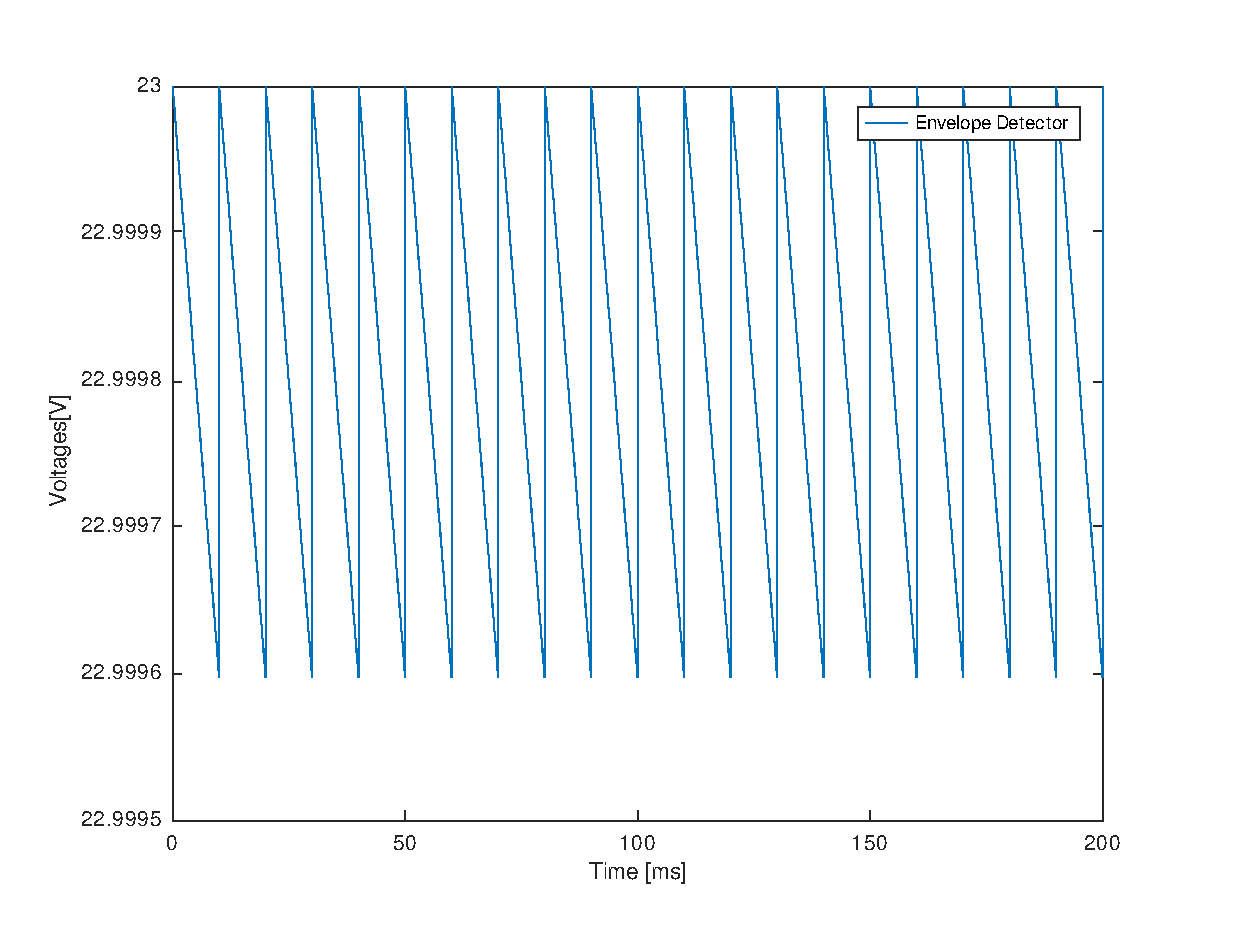
\includegraphics[width = 8cm]{EnvelopeDetector.eps} 
\caption{Output Voltage in Envlope Detector}
\label{fig:first}
\end{figure}

\begin{figure}[H] 
\centering
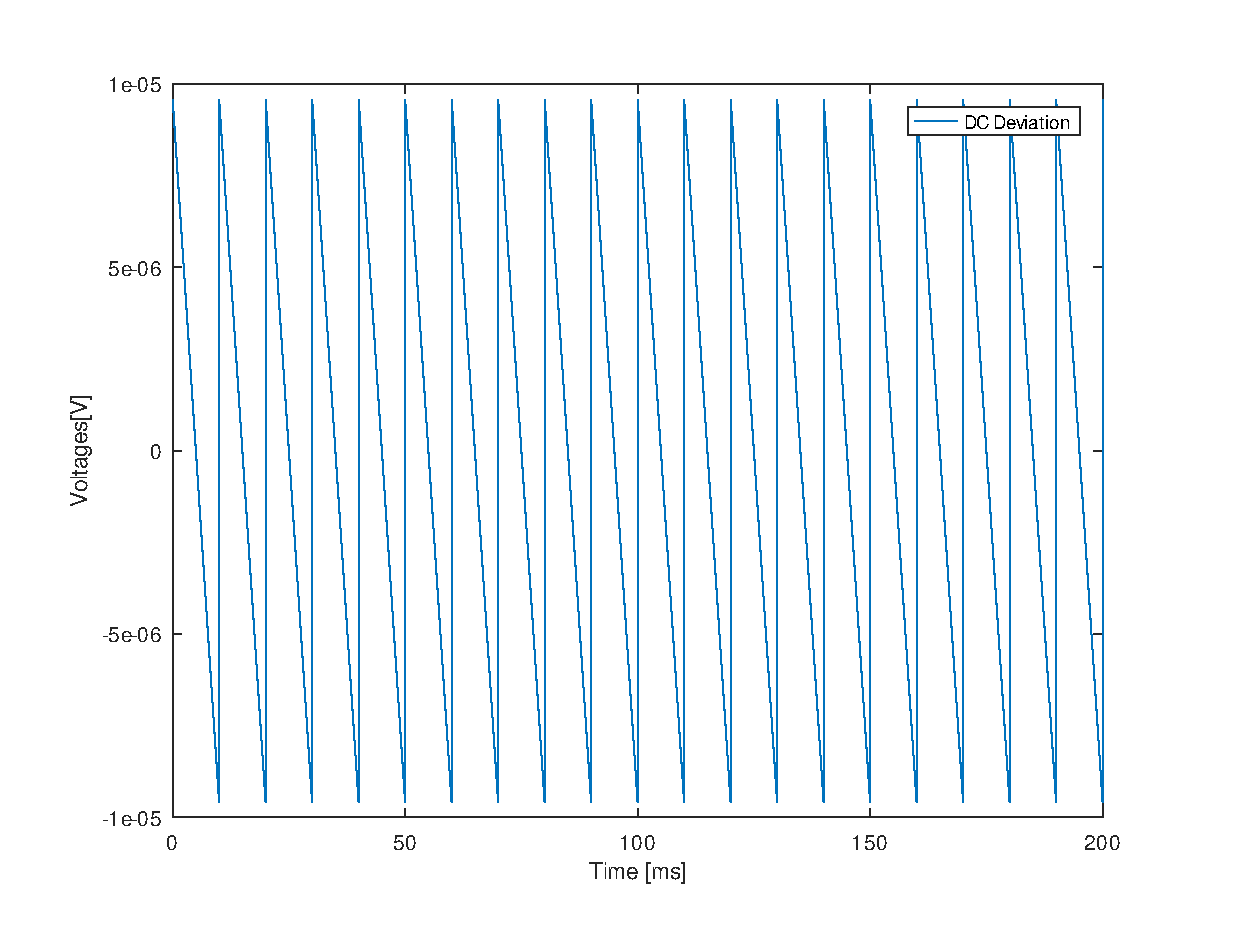
\includegraphics[width = 8cm]{DCDeviation.eps} 
\caption{Output DC Deviation}
\label{fig:first}
\end{figure}

\begin{figure}[H] 
\centering
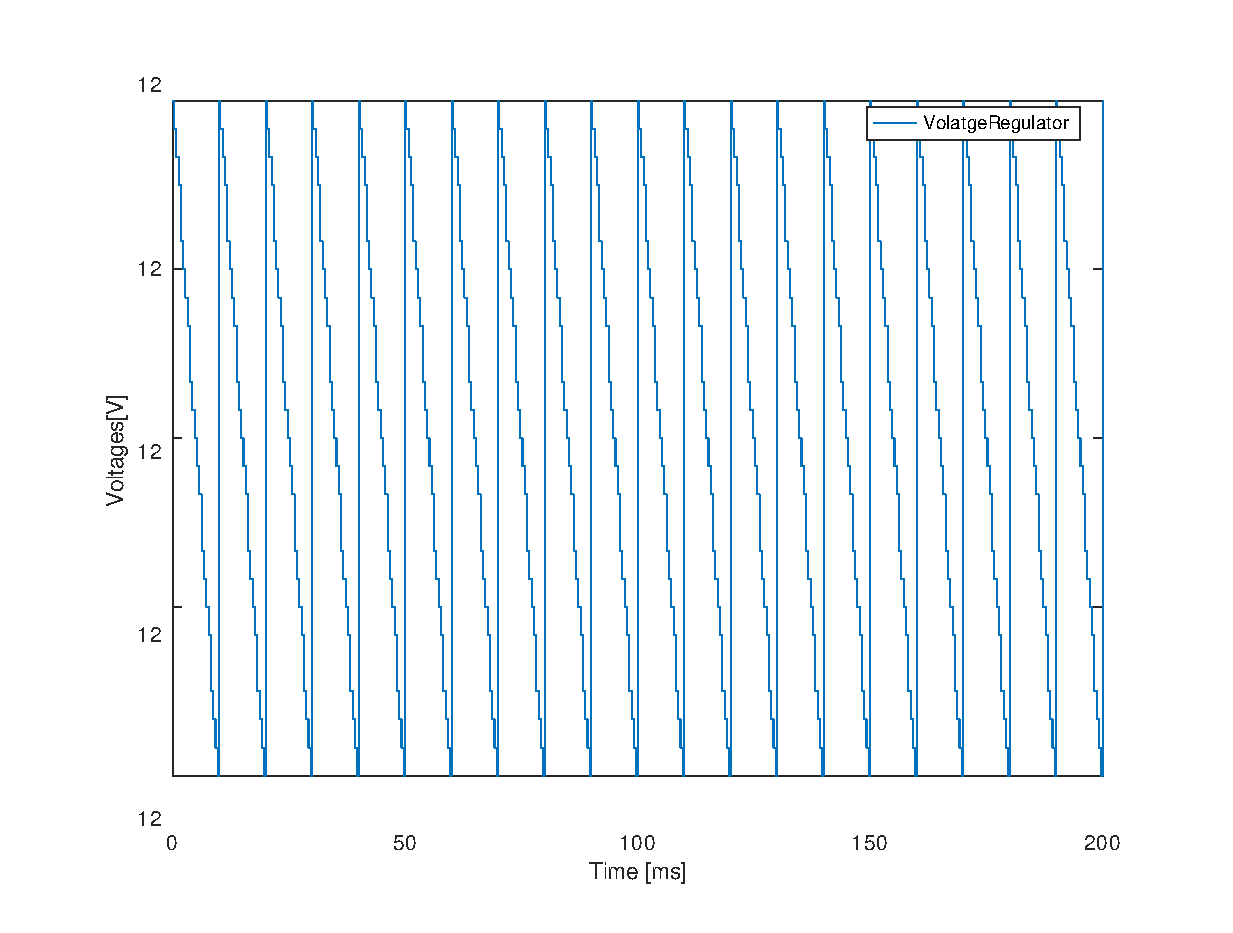
\includegraphics[width = 8cm]{VoltageRegulator.eps} 
\caption{Output Voltage}
\label{fig:first}
\end{figure}


